\documentclass[12pt,a4paper]{article}

\usepackage[left=3.00cm, right=2.00cm, top=2.00cm, bottom=2.00cm]{geometry}
\usepackage{lmodern}
\usepackage[utf8]{inputenc}
\usepackage[brazil]{babel}

\usepackage{amssymb}
\usepackage{amsmath}
\usepackage{amsfonts}
\usepackage{pgfplots}
\pgfplotsset{compat=1.16}

\usepackage{graphicx}
\usepackage{indentfirst}
\usepackage{booktabs}
\usepackage{fancyvrb}

\usepackage{array}
\newcolumntype{L}[1]{>{\raggedright\let\newline\\\arraybackslash\hspace{0pt}}m{#1}}
\newcolumntype{C}[1]{>{\centering\let\newline\\\arraybackslash\hspace{0pt}}m{#1}}
\newcolumntype{R}[1]{>{\raggedleft\let\newline\\\arraybackslash\hspace{0pt}}m{#1}}

\usepackage[numbers]{natbib}
\usepackage{url}
\bibliographystyle{plainnat}

\usepackage{setspace}
\onehalfspacing

\author{Pablo Cecilio Oliveira\\
	Alexander Cristian}
\title{Algorítimos e Estrutura de Dados III\\
	Primeiro Trabalho Prático - Hipercampos}
\date{}

\begin{document}
\maketitle

\section{Introdução}

Na Ciência da Computação, o estudo de algorítimos para resolução de problemas geométricos é conhecido como Geometria Computacional. De forma geral, o objetivo deste ramo é resolver de maneira eficiente utilizando o menor número possível de operações sobre os elementos geométricos elementares.\cite{wiki:compgeo}

Dentre os problemas geométricos, temos um conhecido como ''Hipercampos'', o qual pode ser visto como desafio em maratonas de programação\cite{uri:hipercampo}. Neste trabalho, é apresentado a solução para esse problema por meio de um algorítimo contido em um programa desenvolvido na linguagem em C.

\subsection{Hipercampos, especificação do problema}

No problema de Hipercampos, um plano cartesiano em $\mathbb{R}^2$ possui duas ''âncoras'', dois pontos $A$ e $B$, onde o eixo $Y$ das duas âncoras são iguais a zero, ou seja $A=(X_A ,0)$ e $B=(X_B , 0)$. Os valores do eixo $X$ das âncoras variam de $X_A$ até $X_B$, formando assim um segmento de reta horizontal, tal que $0 < X_A < X_B \leqslant 10^4$. (Fig. \ref{fig:entrada})

\begin{figure}[!h]
	\caption{Exemplo de entrada para o problema.}
	\label{fig:entrada}
	\centering
	\begin{tikzpicture}[baseline]
	\pgfplotsset{width=8.5cm}
	\begin{axis}[
	title={},
	xmin=0, xmax=100,
	ymin=0, ymax=100,
	xtick={0,20,40,60,80,100},
	ytick={0,20,40,60,80,100},
	xmajorgrids=true,
	ymajorgrids=true,
	grid style=dashed,
	%legend style={draw=none},
	]
	
	\addplot[color=black,only marks,mark=square*,mark size=2.9pt]
	coordinates{(10,0)(50,0)};	
	
	\addplot[color=black,only marks,mark size=2.9pt]
	coordinates{
		(4,29)
		(15,15)
		(25,25)
		(35,14)
		(36,30)
		(45,6)
		(26,20)
		(21,10)
		(28,5)
		(40,24)
		(65,16)
		(80,75)
		%(50,62)
		(5,90)
		(60,50)
	};
	\legend{Âncoras}
	\end{axis}
	\end{tikzpicture}
	\footnotesize \\Fonte: autores
\end{figure}

Ao plano cartesiano também somam-se um conjunto $P$ de $N$ pontos $(X_i,Y_i)$, sendo que $N (1 \leqslant N \leqslant 100)$. Os pontos do conjunto $P$ podem ter suas coordenadas variando entre $0$ até $10^4$, ou seja, $0 < X_i,Y_i \leqslant 10^4$.

O objetivo do problema de Hipercampos é ligar os pontos contidos em $P$ às âncoras $X_A$ e $X_B$, formando assim o máximo número de triângulos sem que esses se interceptem (Fig. \ref{fig:solucionando}). E para esse proposito é apresentado um algorítimo contido no programa apresentado neste trabalho.

\begin{figure}[!h]
\caption{Hipercampos, solucionando.}
\label{fig:solucionando}
\begin{tikzpicture}[baseline]
	\pgfplotsset{width=8.3cm}
	\begin{axis}[
	title={},
	xmin=0, xmax=100,
	ymin=0, ymax=100,
	xtick={0,20,40,60,80,100},
	ytick={0,20,40,60,80,100},
	xmajorgrids=true,
	ymajorgrids=true,
	grid style=dashed,
	%legend style={draw=none},
	]	
	
	\addplot+[sharp plot,color=black,mark size=2.9pt]
	coordinates{
		(10,0)(4,29)(50,0)
		(10,0)(15,15)(50,0)
		(10,0)(25,25)(50,0)
		(10,0)(35,14)(50,0)
		(10,0)(36,30)(50,0)
		(10,0)(45,6)(50,0)
		(10,0)(26,20)(50,0)
		(10,0)(21,10)(50,0)
		(10,0)(28,5)(50,0)
		(10,0)(40,24)(50,0)
		(10,0)(65,16)(50,0)
		(10,0)(80,75)(50,0)
		%(10,0)(50,62)(50,0)
		(10,0)(5,90)(50,0)
		(10,0)(60,50)(50,0)
	};
	\end{axis}
\end{tikzpicture}
\begin{tikzpicture}[baseline]
	\pgfplotsset{width=8.3cm}
	\begin{axis}[
	title={},
	xmin=0, xmax=100,
	ymin=0, ymax=100,
	xtick={0,20,40,60,80,100},
	ytick={0,20,40,60,80,100},
	xmajorgrids=true,
	ymajorgrids=true,
	grid style=dashed,
	%legend style={draw=none},
	]	
	
	\addplot+[sharp plot,color=black,mark size=2.9pt]
	coordinates{
		(10,0)(28,5)(50,0)
		(10,0)(35,14)(50,0)
		(10,0)(40,24)(50,0)
		(10,0)(60,50)(50,0)
		(10,0)(80,75)(50,0)
	};
	\end{axis}
\end{tikzpicture}
\footnotesize \hphantom{space}Fonte: autores
\end{figure}

\subsection{Visão geral sobre o funcionamento do programa}

O programa desenvolvido recebe por parâmetro a entrada de um arquivo contendo em sua primeira linha um número $N$ de pontos no plano $\mathbb{R}^2$ e as coordenadas do eixo $X$ das âncoras $A$ e $B$, respectivamente. As linhas subsequentes a primeira correspondem às coordenadas dos $N$ pontos do conjunto $P$ a ser solucionado.

O algorítimo então processa esses dados retornando uma solução que pode ser verificada por meio de dois arquivos também gerados por um parâmetro: um contendo o número de triângulos possíveis e o outro em forma de uma imagem renderizada como ''gráfico vetorial escalável'' (Scalable Vector Graphics, ou ''.svg'')\footnote{Trata-se de uma linguagem XML para descrever de forma vetorial desenhos e gráficos bidimensionais.}. Um terceiro arquivo em ''.svg'' é gerado contendo a entrada original dos dados para referência.

O programa é executado no prompt de comando e recebe as passagens de parâmetro dos arquivos de entrada e saída:

\begin{figure}[!h]
\centering
\begin{BVerbatim}
$ ./hcamp -i [input] -o [output]
\end{BVerbatim}
\end{figure}

A entrada e solução renderizada pode ser vista no exemplo da Figura \ref{fig:inrend}.

\begin{figure}[!h]
	\caption{Entrada e saída renderizadas.}
	\label{fig:inrend}
	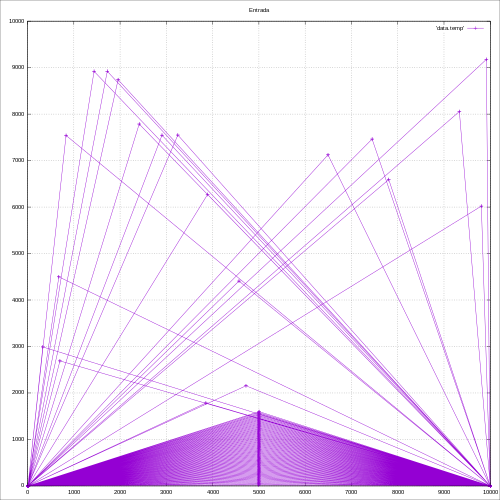
\includegraphics[width=75mm]{input.png}
	\hfill
	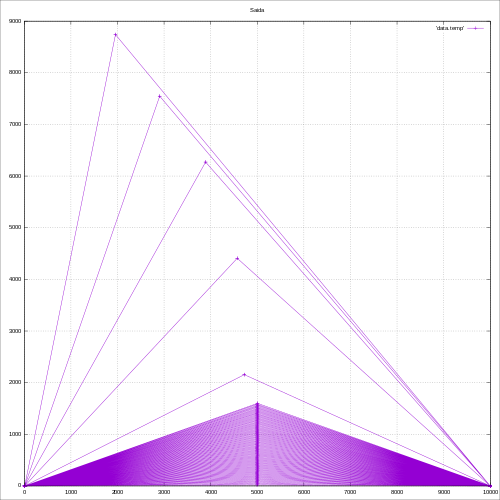
\includegraphics[width=75mm]{output.png}\\
	\footnotesize Fonte: autores
\end{figure}

\section{Implementação}

O método em questão usado para resolver esse problema se baseia na exploração do sistema de coordenadas baricêntricas e na orientação dos segmentos de retas formados pela conexão dos pontos. Portanto em primeiro lugar é verificada a orientação das retas para isolar os casos em que elas se interceptam ou são colineares.

Logo em seguida precisa-se saber quando um ponto esta contido em um triangulo. Uma solução simples seria traçar uma reta que segue horizontalmente para a direita, e depois fazendo comparações para saber quantas vezes ela intercepta o polígono formado, se o resultado for um número par o ponto está fora, se for impar ele está dentro. Porem isso levaria o programa a executar muitas operações, então evoluindo desse conceito chegamos a uma solução usando as coordenadas baricêntricas, onde é verificado em qual lado do meio plano criado pelas arestas está o ponto.

Verifica por meio da expressão de orientação da reta:

\begin{figure}[!h]
	\caption{Determinando o ponto interno ao triângulo}
	\begin{tikzpicture}[baseline]
	\pgfplotsset{width=8cm}
	\begin{axis}[
	title={},
	xmin=0, xmax=80,
	ymin=0, ymax=80,
	xtick={0,20,40,60,80,100},
	ytick={0,20,40,60,80,100},
	grid style=dashed,
	%legend style={draw=none},
	]	
	
	\addplot+[color=black,mark size=2.9pt]
	coordinates{
		(10,0)(40,75)
	};
	\addplot[color=red,mark size=2.9pt]
	coordinates{
		(10,0)(40,50)
	};
	
	\addplot[mark=*] coordinates {(40,50)} node[pin=310:{$PQR>0$}]{} ;
	
	\end{axis}
	\end{tikzpicture}
	\begin{tikzpicture}[baseline]
	\pgfplotsset{width=8cm}
	\begin{axis}[
	title={},
	xmin=0, xmax=80,
	ymin=0, ymax=80,
	xtick={0,20,40,60,80,100},
	ytick={0,20,40,60,80,100},
	grid style=dashed,
	%legend style={draw=none},
	]	
	
	\addplot+[color=black,mark size=2.9pt]
	coordinates{
		(70,0)(40,75)
	};
	\addplot[color=red,mark size=2.9pt]
	coordinates{
		(70,0)(40,50)
	};
	
	\addplot[mark=*] coordinates {(40,50)} node[pin=250:{$PQR<0$}]{} ;
	
	\end{axis}
	\end{tikzpicture}
	\footnotesize{\\Fonte: autores}
\end{figure}

\[(y2-y1) (x3-x2) - (y3-y2) (x2-x1)\]

Se os pontos são colineares, e a orientação do triangulo (horário ou anti-horário)

\begin{table}[!htbp]
	\centering
	\caption{Funções do programa}
	\renewcommand{\arraystretch}{1.5}
	\begin{tabular}{L{3cm} L{10cm} c}
		\toprule 
		Funções & Finalidade & Complexidade* \\ 
		\midrule
		$debug()$ & Função que verifica a condição para retorno de possíveis bugs no programa. & $O(1)$ \\
		$create()$ & Inicializa a Lista encadeada. & $O(1)$ \\
		$insere()$ & Insere os dados em uma lista encadeada. & $O(1)$ \\
		$printCJT()$ & Imprime uma Lista encadeada. & $O(n)$ \\
		$sizeCJT()$ & Retorna o tamanho da lista encadeada. & $O(n)$ \\
		$dump()$ & Libera a memoria alocada pela lista. & $O(n)$ \\
		$isEmpty()$ & Verifica se uma lista encadeada está vazia. & $O(1)$ \\
		$openFILE()$ & Abre o arquivo solicitado e transfere os dados para uma lista encadeada. & $O(n)$ \\
		$saveFILE()$ & Salva a solução do problema em um arquivo. & $O(1)$ \\
		$chkFILE()$ & Verifica por possíveis erros de entrada em um arquivo. & $O(1)$ \\
		$showerro()$ & Retorna possíveis erros no arquivo de entrada. & $O(1)$ \\
		$ask()$ & Solicita a confirmação do usuário caso erros de entrada sejam encontrados. & $O(1)$ \\
		$cpyCJT()$ & Copia os dados de uma lista encadeada para outra lista encadeada. & $O(1)$ \\
		$PQR()$ & Algorítimo de orientação do ponto em relação a reta da ancora. & $O(1)$ \\
		$findMAX()$ & Função recursiva que determina o maior conjunto de pontos que se encontram dentro do triângulo formado pelas ancoras e um ponto $(x,y)$.  & $O(n)$ \\
		$soluciona()$ \newline $solucao()$ & Funções de chamada e retorno para a execução do algorítimo & $O(1)$ \\
		$plotGraph()$ & PIPE para o gnuplot com a finalidade de renderizar os arquivos .svg contendo respectivamente, a entrada e saída da solução do problema.  & $O(n)$ \\ 
		\bottomrule
		\footnotesize Fonte: autores
	\end{tabular}
\end{table}

\section{Análise de Complexidade}

\[ \begin{split}
f(n) &= 11 + (n+1)*\frac{n}{n-1}+\frac{n}{2}*\frac{1}{2n}+n+\frac{n}{2}+4n \\
f(n) &= 11 + \frac{n^2+n}{n-1}+\frac{n}{4n}+\frac{n}{2}+5n \\
f(n) &= \frac{26n^2+27n-45}{4(n-1)}
\end{split} \]

\[T(n)=aT(\frac{n}{b})+f(n)\]


\begin{center}
	\begin{tikzpicture}
	\begin{axis}[
	title={Figura 5: Tempo de execução do algoritimo},
	xmin=0, xmax=100,
	ymin=0, ymax=360,
	xlabel={Dados de entrada},
	ylabel={Tempo de execução},
	xtick={0,20,40,60,80,100},
	ytick={0,60,120,180,240,300,360},
	grid style=dashed,
	%legend style={draw=none},
	]
	
	\end{axis}
	\end{tikzpicture}
	\footnotesize{\\Fonte: autores}
\end{center}

\section{Considerações finais}

O Trabalho computacional 1 da disciplina foi uma grande oportunidade para aprender sobre grafos e LCS, que rodeiam o algoritmo ótimo para a solução desse problema, o que é a introdução para programação dinâmica e acreditamos ser o intuito desse trabalho, também proporcionou um contato maior com a analise de complexidade do algoritmo. 

Um dos maiores problemas no desenvolvimento foi encontrar um algoritmo que possuísse um comportamento adequado quando a entrada de valores é muito grande. Apesar da forte base matemática de nossos métodos, em alguns casos eles podem levar a uma falta de precisão, porque o sistema de números de ponto flutuante tem tamanho limitado e na maioria das vezes lida com aproximações. O problema ocorre às vezes quando um ponto p deve estar exatamente na borda de um triângulo, as aproximações levam a falhar no teste. 

Para a construção de gráficos que auxiliam em uma melhor visualização do trabalho foi necessário o gnuplot.

\pagebreak

\begin{flushleft}
	\nocite{*}
	\bibliography{tp_hcamp}
\end{flushleft}

\end{document}
